\subsection{Framework} \label{framework}
\begin{figure}[H]
	\centering
	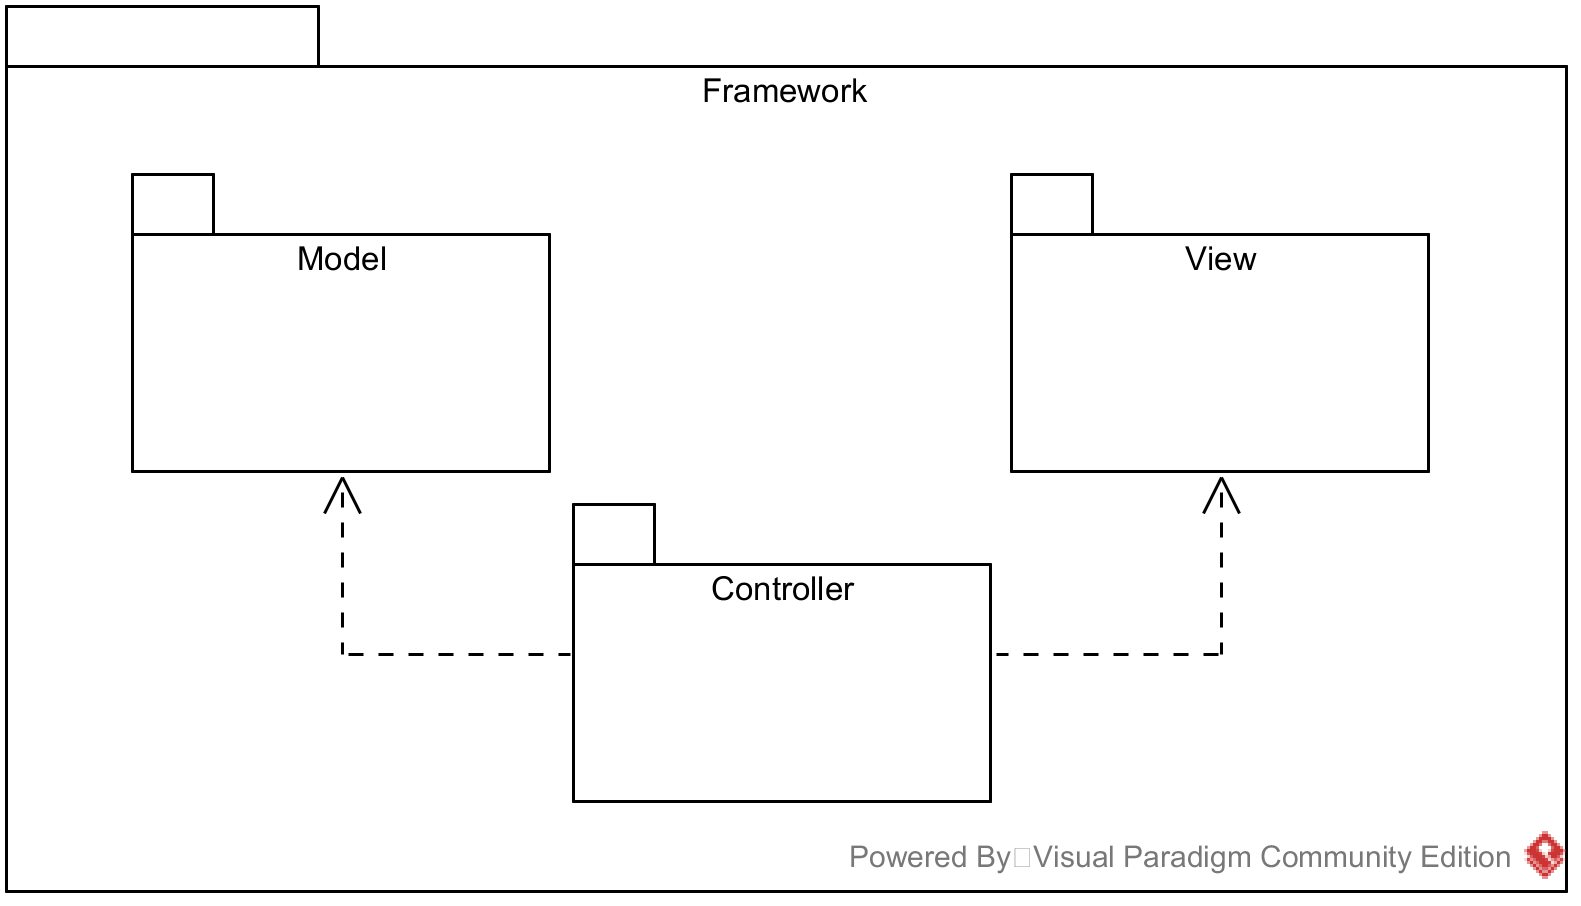
\includegraphics[width=15cm]{./diagrammi/framework.png}
	\caption{Componente Framework}
\end{figure}
\glossario{Framework} è il \glossario{package} base per la corrispondente parte di progetto. È composto dai package Model, View e Controller, in relazione tra loro secondo il \glossario{design pattern} adottato \glossario{MVC}, nella sua versione pull.

\setclass{Framework::Model}
\subsubsection[::Model]{\class} \label{\class}
\begin{figure}[H]
	\centering
	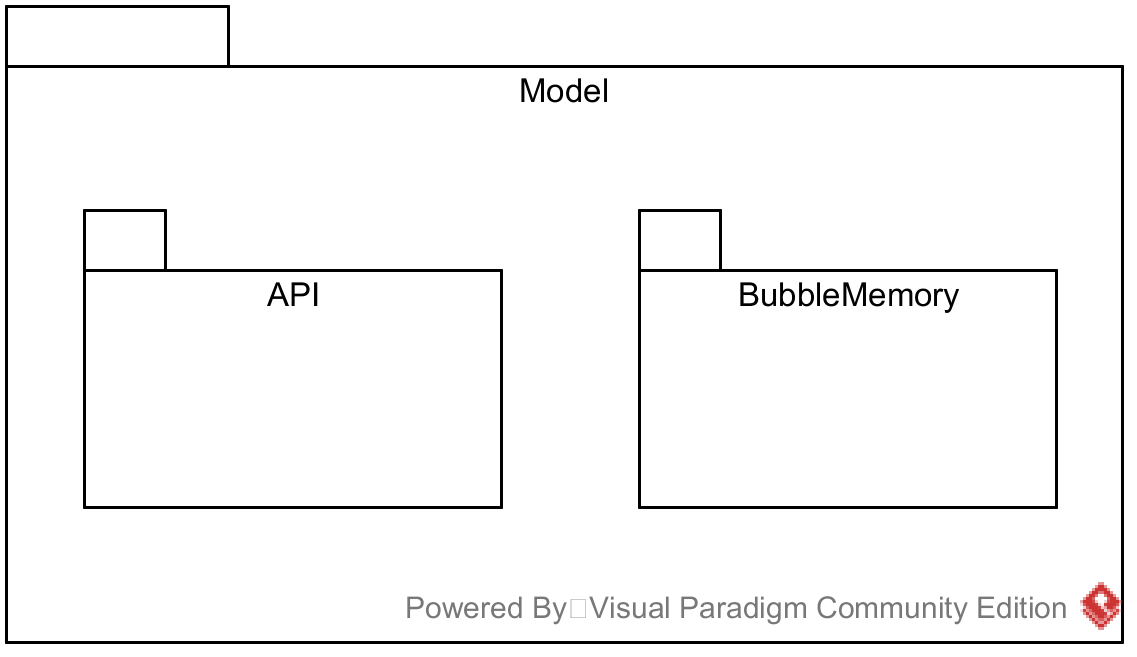
\includegraphics[width=10cm]{./diagrammi/framework/model.png}
	\caption{Componente \class}
\end{figure}
Contiene la business logic del framework, ed è composto dai package API e BubbleMemory.

\setclass{Framework::Model::BubbleMemory::BubbleMemory}
\paragraph[::BubbleMemory::BubbleMemory]{\class}\mbox{}\\ \label{class}
\begin{figure}[H]
	\centering
	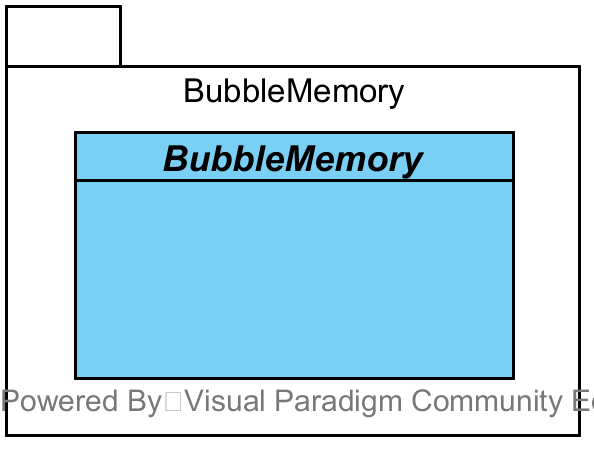
\includegraphics[width=7cm]{./diagrammi/framework/model/bubblememory.png}
	\caption{Classe \class}
\end{figure}

\textbf{Descrizione:}\\
Classe astratta che rappresenta la memoria della bubble.

\textbf{Utilizzo:}\\
Viene utilizzata per dare un'interfaccia comune per vari possibili sviluppi della memoria della bubble.

\textbf{Classi ereditate:}
\begin{itemize}
	\item \code{EventEmitter}.
\end{itemize}

\textbf{Sottoclassi:}
\begin{itemize}
	\item \coderef{Framework::Model::API::ExternalAPI::ExternalAPIStore}.
\end{itemize}

%\textbf{Attributi:}
%
%\textbf{Metodi:}

\setclass{Framework::Model::API}
\paragraph[::API]{\class}\mbox{}\\ \label{\class}
\begin{figure}[H]
	\centering
	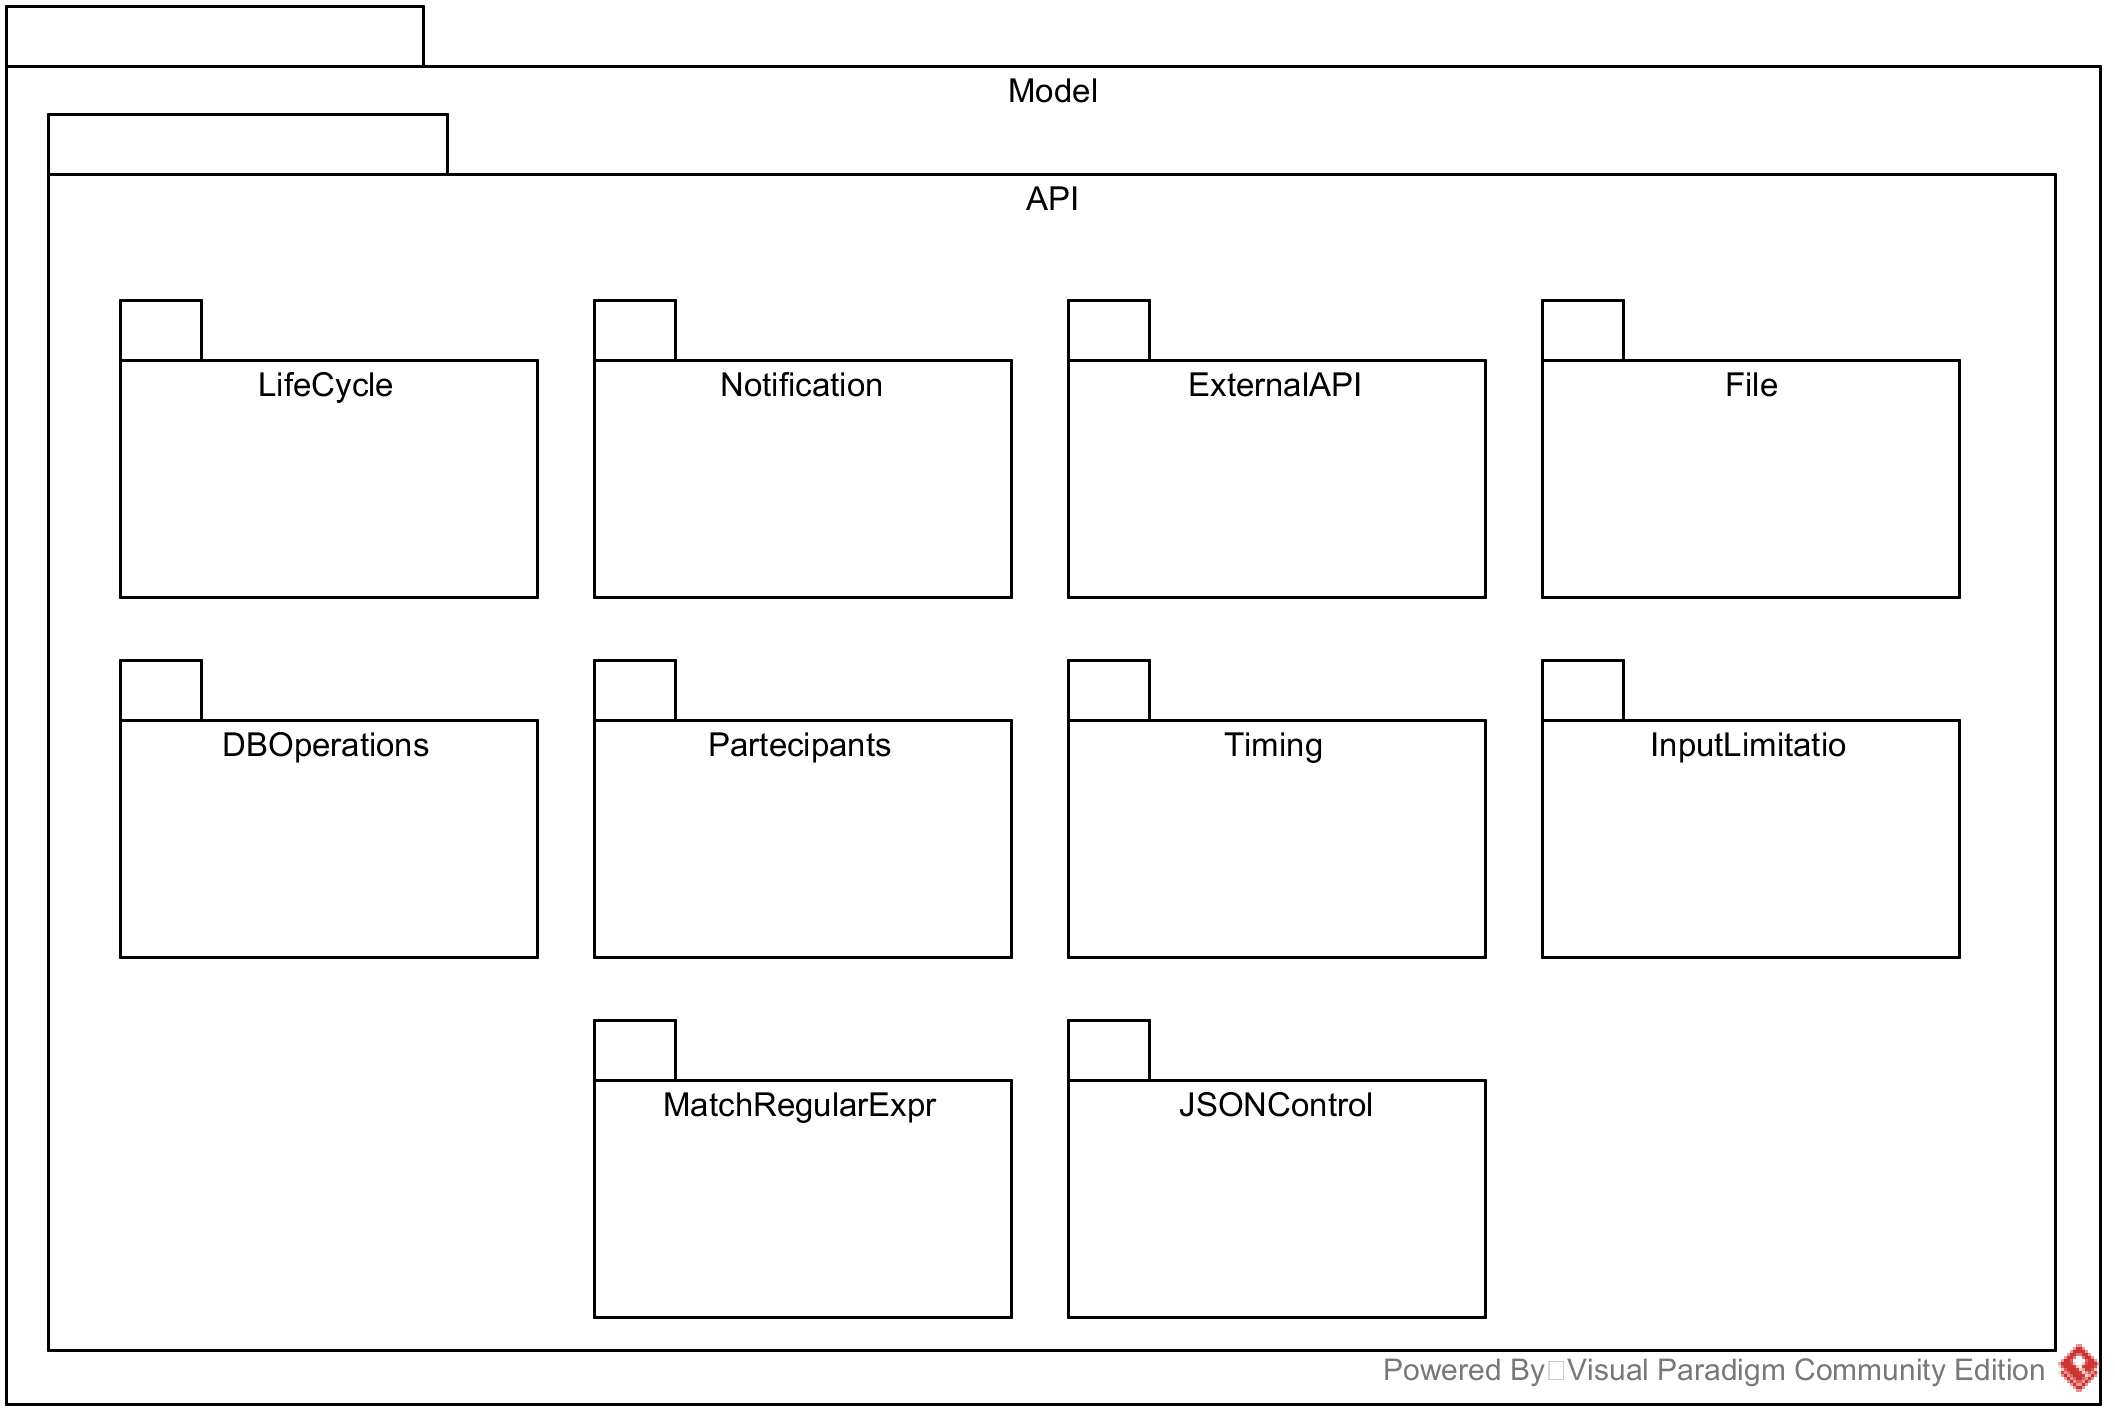
\includegraphics[width=15cm]{./diagrammi/framework/model/api.png}
	\caption{Componente \class}
\end{figure}
Questo componente ha lo scopo di racchiudere in sè tutte le funzionalità logiche offerte dal framework. Non vi sono relazioni tra esse per mantenere una forte indipendenza.

\setclass{Framework::Model::API::LifeCycle::LifeCycle}
\subparagraph[::LifeCycle::LifeCycle]{\class}\mbox{}\\ \label{\class}
\begin{figure}[H]
	\centering
	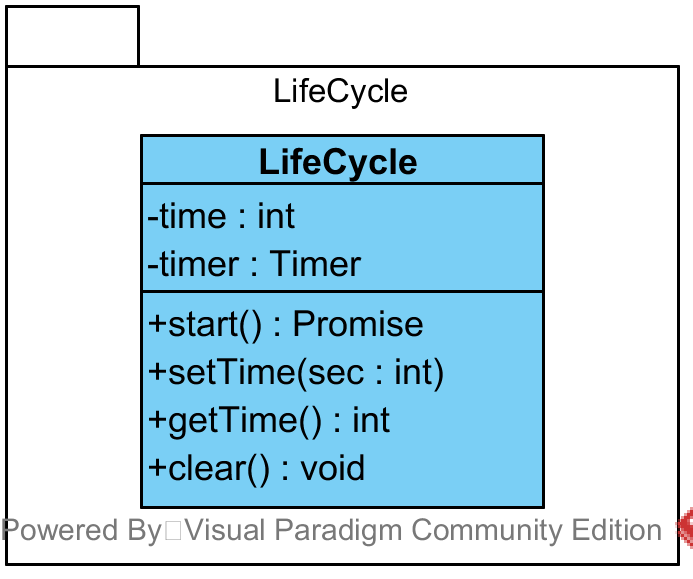
\includegraphics[width=7cm]{./diagrammi/framework/model/api/lifecycle.png}
	\caption{Classe \class}
\end{figure}

\textbf{Descrizione:}\\
Classe che permette di inizializzare e avviare un timer.

\textbf{Utilizzo:}\\
Viene utilizzata per definire il tempo di vita di una bubble e avviare il timer che ne determina la fine.

%\textbf{Classi ereditate:}

%\textbf{Sottoclassi:}

\textbf{Attributi:}
\begin{itemize}
	\item \field{- time: int}: durata in secondi del timer;
	\item \field{- timer: Timeout}: riferimento al timer.
\end{itemize}

\textbf{Metodi:}
\begin{itemize}
	\item \method{+ start(): Promise}: restituisce una promise in cui il timer viene avviato;
	\item \method{+ getTime(): int}: restituisce il tempo impostato;
	\item \method{+ setTime(sec: int): void}: permette di settare il tempo:
	\begin{itemize}
		\item \param{sec: int}: durata in secondi del timer.
	\end{itemize}
	\item \method{+ clear(): void}: permette di fermare il timer e resettarlo.
\end{itemize}

\setclass{Framework::Model::API::Notification::WebNotification}
\subparagraph[::Notification::WebNotification]{\class}\mbox{}\\ \label{\class}
\begin{figure}[H]
	\centering
	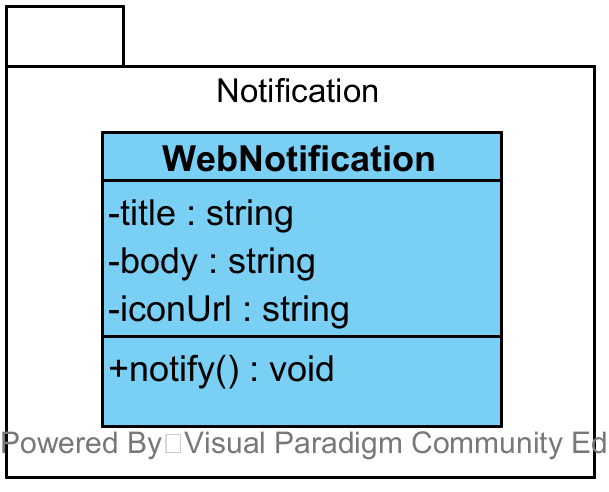
\includegraphics[width=7cm]{./diagrammi/framework/model/api/notification.png}
	\caption{Classe \class}
\end{figure}

\textbf{Descrizione:}\\
Classe che permette di creare notifiche.

\textbf{Utilizzo:}\\
Viene utilizzata per creare e mostrare delle notifiche all'utente utilizzatore della bubble.

%\textbf{Classi ereditate:}

%\textbf{Sottoclassi:}

\textbf{Attributi:}
\begin{itemize}
	\item \field{- title: string}: titolo della notifica;
	\item \field{- body: string}: messaggio della notifica;
	\item \field{- iconUrl: string}: URI dell'icona della notifica.
\end{itemize}

\textbf{Metodi:}
\begin{itemize}
	\item \method{+ notify(): void}: se sono state attivate, crea una notifica.
\end{itemize}

\setclass{Framework::Model::API::ExternalAPI}
\subparagraph[::ExternalAPI]{\class}\mbox{}\\ \label{\class}
\begin{figure}[H]
	\centering
	\includegraphics[width=15cm]{./diagrammi/framework/model/api/externalapi.png}
	\caption{Componente \class}
\end{figure}
All'interno di questo componente sono definite le classi necessarie per effettuare richieste ad API esterne.

\setclass{Framework::Model::API::ExternalAPI::ExternalAPI}
\subsubparagraph[::ExternalAPI]{\class}\mbox{}\\ \label{\class}
%\begin{figure}[H]
%	\centering
%	\includegraphics[width=7cm]{./diagrammi/framework/model/api/externalapi/externalapi.png}
%	\caption{Classe \class}
%\end{figure}

\textbf{Descrizione:}\\
Classe che permette di effettuare richieste a API esterne.

%\textbf{Utilizzo:}\\
%Viene utilizzata per richiedere informazioni da fonti esterne alla bubble, integrandole in essa.

\textbf{Classi ereditate:}
\begin{itemize}
	\item \code{React::Component}
\end{itemize}
%\textbf{Sottoclassi:}

\textbf{Attributi:}
\begin{itemize}
	\item \field{- informations: JSON}: risposta ricevuta dopo la richiesta;
	\item \field{- myurl: string}: URI dell'API;
	\item \field{- items: string[]}: array contentente \texttt{informations} suddiviso in stringhe.
\end{itemize}

\textbf{Metodi:}
\begin{itemize}
	\item \method{+ ExternalAPI(props: Object[])}: costruttore della classe, assegna le proprietà:
	\begin{itemize}
		\item \param{props: Object[]}: array generico contenente le proprietà da assegnare;
	\end{itemize}
	\item \method{+ getInitialState(): Object}: ritorna lo stato iniziale della classe, sotto forma di oggetto;
	\item \method{+ componentWillMount(): void}: aggiorna in memoria la risposta ricevuta;
	\item \method{+ componentDidMount(): void}: effettua la richiesta vera e propria.
\end{itemize}

\setclass{Framework::Model::API::ExternalAPI::ExternalAPIStore}
\subsubparagraph[::ExternalAPIStore]{\class}\mbox{}\\ \label{\class}
%\begin{figure}[H]
%	\centering
%	\includegraphics[width=7cm]{./diagrammi/framework/model/api/externalapi/externalapistore.png}
%	\caption{Classe \class}
%\end{figure}

\textbf{Descrizione:}\\
Classe che permette di salvare una risposta API.

%\textbf{Utilizzo:}\\
%Viene utilizzata per salvare nella memoria della bubble le informazioni ricevute da \cref{Framework::Model::API::ExternalAPI::ExternalAPI}.

\textbf{Classi ereditate:}
\begin{itemize}
	\item \code{\cref{Framework::Model::BubbleMemory::BubbleMemory}}
\end{itemize}
%\textbf{Sottoclassi:}

\textbf{Attributi:}
\begin{itemize}
	\item \field{- items: string[]}: informazioni della risposta come array di stringhe;
	\item \field{- itemNumber: int}: quantità di informazioni memorizzate;
\end{itemize}

\textbf{Metodi:}
\begin{itemize}
	\item \method{+ ExternalAPIStore()}: costruttore della classe, inizializza \texttt{items} come array vuoto e \texttt{itemNumber} a zero;
	\item \method{+ addItems(text: string): void}: inserisce la stringa nell'array \texttt{items} e segnala il cambiamento;
	\item \method{+ getItems(): string[]}: ritorna l'array \texttt{items};
	\item \method{+ handleActions(action: string): void}: gestisce alcune azioni frequenti:
	\begin{itemize}
		\item \param{action: string}: nome dell'azione, in maiuscolo e \virgolette{underscore\_case}.
	\end{itemize}
\end{itemize}

%\setclass{Framework::Model::API::Partecipants::Partecipants}
%\subparagraph[::Partecipants::Partecipants]{\class}\mbox{}\\ \label{\class}
%\begin{figure}[H]
%	\centering
%	\includegraphics[width=7cm]{./diagrammi/framework/model/api/partecipants.png}
%	\caption{Classe \class}
%\end{figure}

%\textbf{Descrizione:}\\
%Classe che permette di visualizzare la lista dei partecipanti della bubble e uno storico delle interazioni con essa.

%\textbf{Utilizzo:}\\
%Viene utilizzata per monitorare gli accessi alla bubble.

%\textbf{Classi ereditate:}

%\textbf{Sottoclassi:}

%\textbf{Attributi:}
%\begin{itemize}
%\end{itemize}
%
%\textbf{Metodi:}
%\begin{itemize}
%\end{itemize}

\setclass{Framework::Model::API::DBOperations::DBOperations}
\subparagraph[::DBOperations]{\class}\mbox{}\\ \label{\class}
\begin{figure}[H]
	\centering
	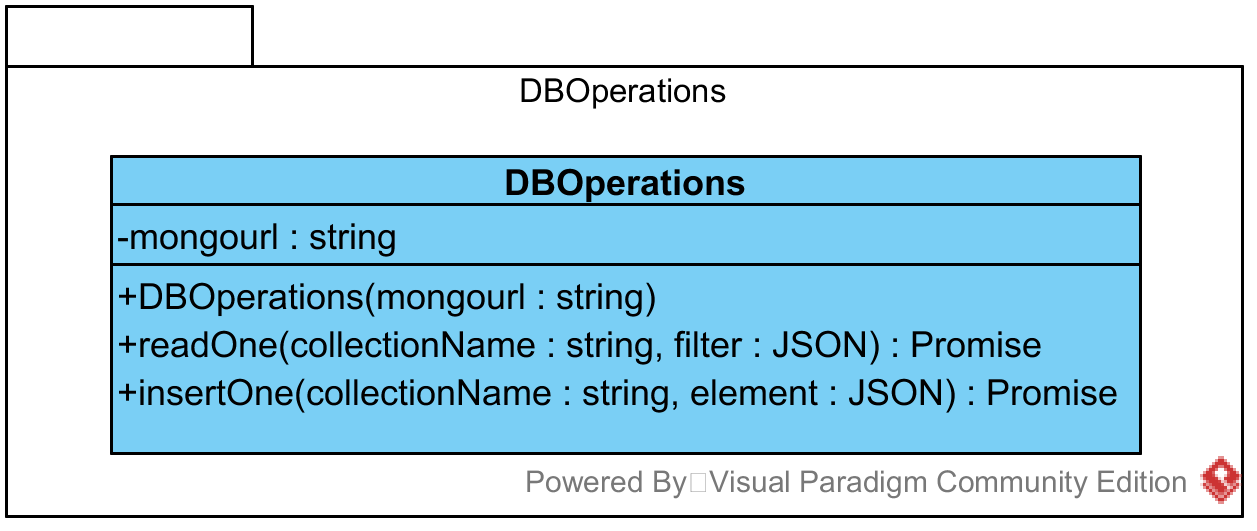
\includegraphics[width=15cm]{./diagrammi/framework/model/api/dboperations.png}
	\caption{Classe \class}
\end{figure}

\textbf{Descrizione:}\\
Classe che permette di effettuare operazioni con un database MongoDB.

\textbf{Utilizzo:}\\
Viene utilizzata per connettere la bubble al database e effettuare operazioni su di esso.

%\textbf{Classi ereditate:}

%\textbf{Sottoclassi:}

\textbf{Attributi:}
\begin{itemize}
	\item \field{- mongourl: string}: indirizzo del database.
\end{itemize}

\textbf{Metodi:}
\begin{itemize}
	\item \method{+ DBOperations(mongoUrl: string)}: costruttore, inizializza \texttt{mongourl}:	
	\begin{itemize}
		\item \param{mongoUrl: string}: indirizzo del database a cui effettuare le connessioni;
	\end{itemize}
	\item \method{+ readOne(collectionName: string, filter: Object): Promise}: effettua una ricerca e ritorna una promise con cui è possibile effettuare operazioni sul risultato:
	\begin{itemize}
		\item \param{collectionName: string}: nome della collezione MongoDB in cui cercare;
		\item \param{filter: Object}: query di ricerca sotto forma di oggetto;
	\end{itemize}
	\item \method{+ insertOne(collectionName: string, element: Object): Promise}: inserisce un elemento nella collezione indicata e ritorna una promise con cui è possibile effettuare operazioni sul risultato:
	\begin{itemize}
		\item \param{collectionName: string}: nome della collezione;
		\item \param{element: Object}: elemento da inserire.
	\end{itemize}
\end{itemize}

%\setclass{Framework::Model::API::InputLimitation::InputLimitation}
%\subparagraph[::InputLimitation::InputLimitation]{\class}\mbox{}\\ \label{\class}
%\begin{figure}[H]
%	\centering
%	\includegraphics[width=7cm]{./diagrammi/framework/model/api/inputlimitation.png}
%	\caption{Classe \class}
%\end{figure}

%\textbf{Descrizione:}\\
%Classe che permette di effettuare controlli dell'input.

%\textbf{Utilizzo:}\\
%Viene utilizzata per controllare e limitare le interazioni con la bubble.

%\textbf{Classi ereditate:}

%\textbf{Sottoclassi:}
%
%\textbf{Attributi:}
%\begin{itemize}
%\end{itemize}
%
%\textbf{Metodi:}
%\begin{itemize}
%\end{itemize}

%\setclass{Framework::Model::API::Timing::Timing}
%\subparagraph[::Timing::Timing]{\class}\mbox{}\\ \label{\class}
%\begin{figure}[H]
%	\centering
%	\includegraphics[width=7cm]{./diagrammi/framework/model/api/timing.png}
%	\caption{Classe \class}
%\end{figure}

%\textbf{Descrizione:}\\
%Classe che permette di pianificare l'esecuzione di azioni ed eventi.

%\textbf{Utilizzo:}\\
%Viene utilizzata per la gestione delle scadenze o di eventi ripetuti in modo automatico.

%\textbf{Classi ereditate:}

%\textbf{Sottoclassi:}
%
%\textbf{Attributi:}
%\begin{itemize}
%\end{itemize}
%
%\textbf{Metodi:}
%\begin{itemize}
%\end{itemize}

%\setclass{Framework::Model::API::File::File}
%\subparagraph[::File::File]{\class}\mbox{}\\ \label{\class}
%\begin{figure}[H]
%	\centering
%	\includegraphics[width=7cm]{./diagrammi/framework/model/api/file.png}
%	\caption{Classe \class}
%\end{figure}

%\textbf{Descrizione:}\\
%Classe che permette di gestire file.

%\textbf{Utilizzo:}\\
%Viene utilizzata per convertire del testo in PDF e salvare dei file.

%\textbf{Classi ereditate:}

%\textbf{Sottoclassi:}
%
%\textbf{Attributi:}
%\begin{itemize}
%\end{itemize}
%
%\textbf{Metodi:}
%\begin{itemize}
%\end{itemize}

%\setclass{Framework::Model::API::JSONControl::JSONControl}
%\subparagraph[::JSONControl::JSONControl]{\class}\mbox{}\\ \label{\class}
%\begin{figure}[H]
%	\centering
%	\includegraphics[width=7cm]{./diagrammi/framework/model/api/jsoncontrol.png}
%	\caption{Classe \class}
%\end{figure}

%\textbf{Descrizione:}\\
%Classe che permette di effettuare un controllo sullo schema di un file JSON.

%\textbf{Utilizzo:}\\
%Viene utilizzata per verificare che il JSON prodotto sia conforme ad uno schema fornito.

%\textbf{Classi ereditate:}

%\textbf{Sottoclassi:}
%
%\textbf{Attributi:}
%\begin{itemize}
%\end{itemize}
%
%\textbf{Metodi:}
%\begin{itemize}
%\end{itemize}

\setclass{Framework::Model::API::MatchRegularExpr::MatchRegularExpr}
\subparagraph[::MatchRegularExpr::MatchRegularExpr]{\class}\mbox{}\\ \label{\class}
\begin{figure}[H]
	\centering
	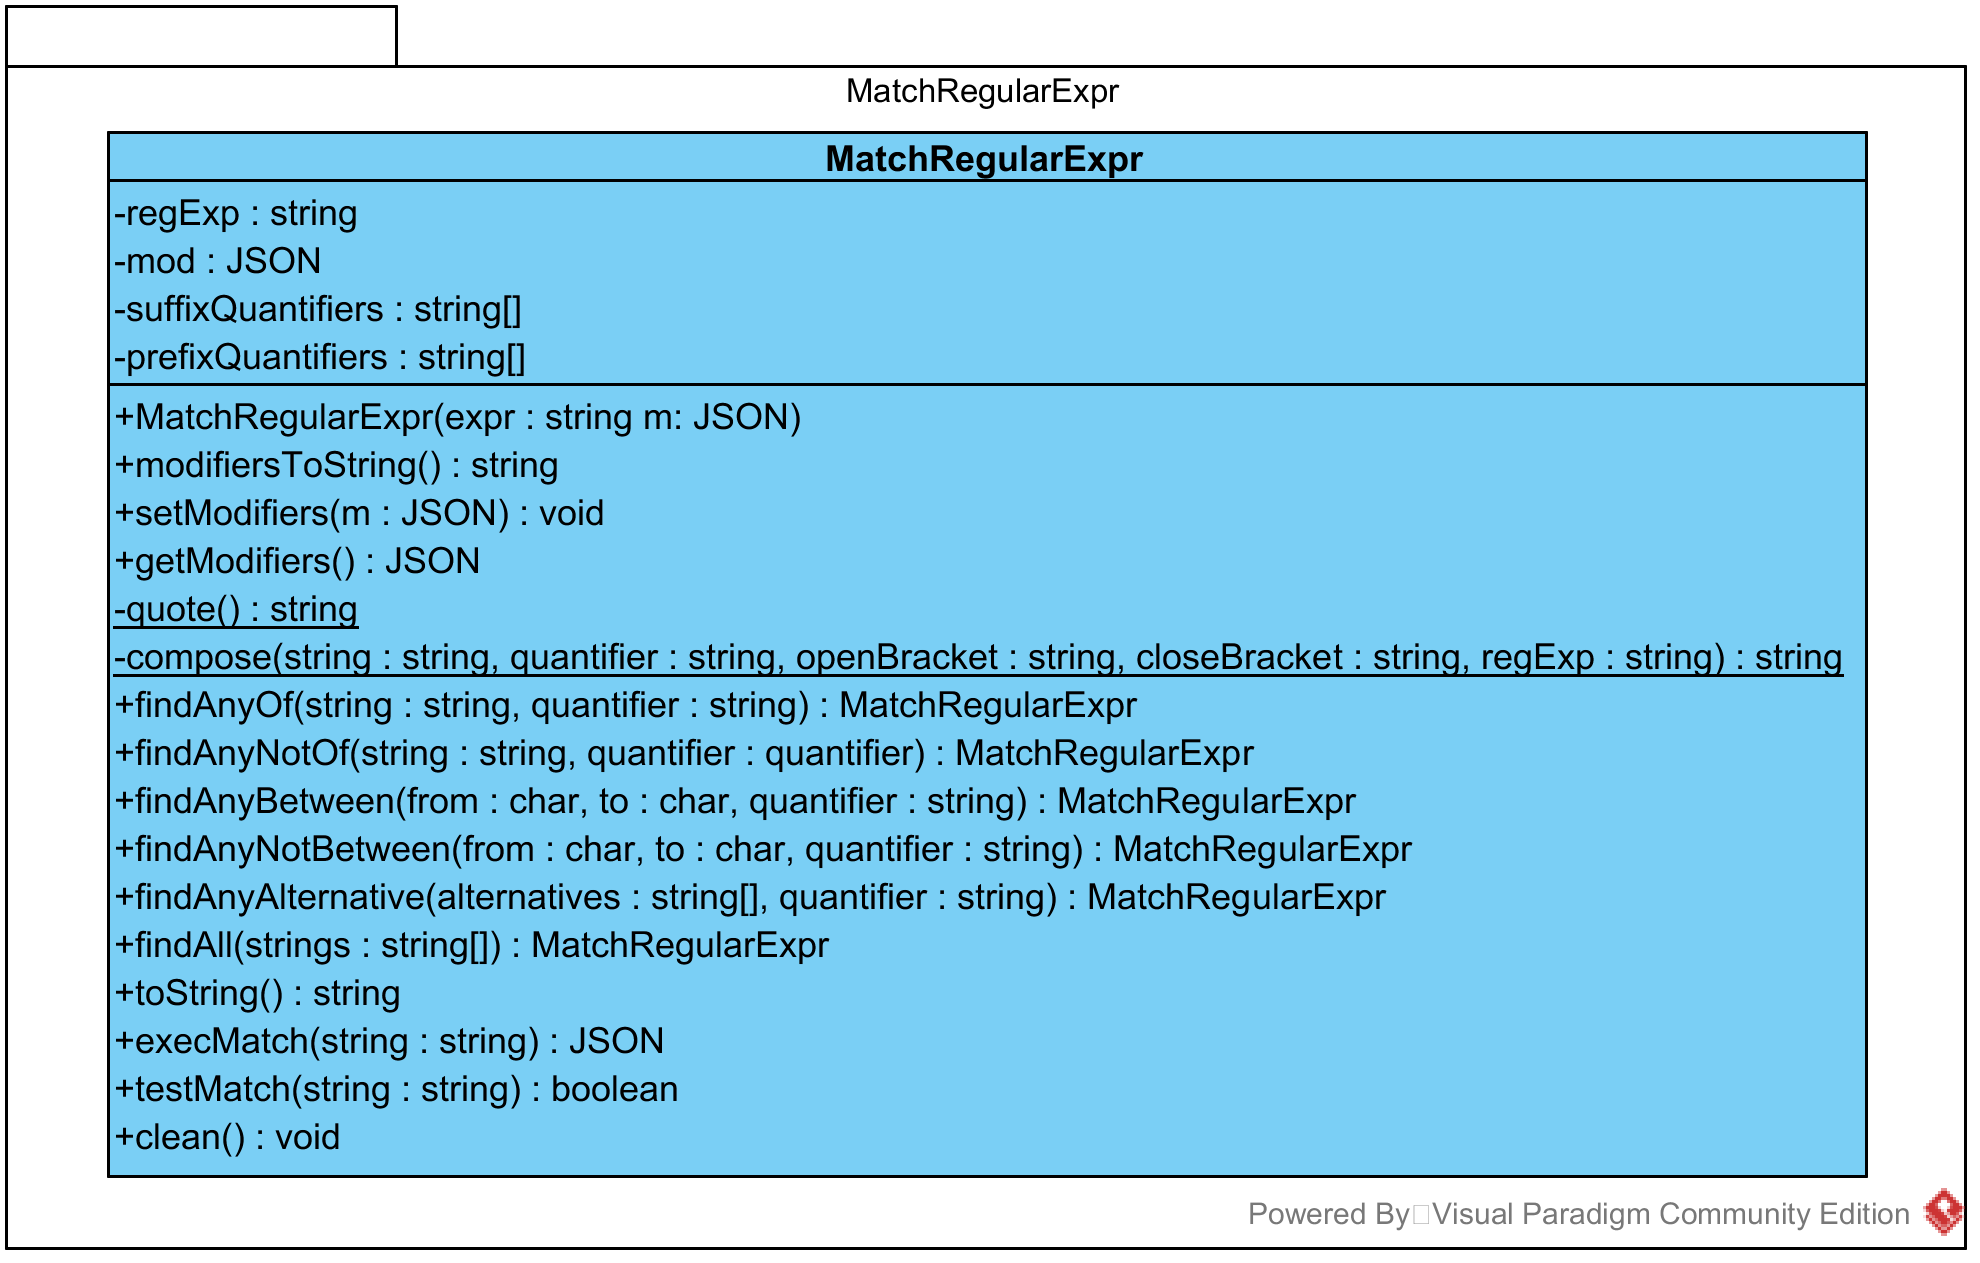
\includegraphics[width=15cm]{./diagrammi/framework/model/api/matchregularexpr.png}
	\caption{Classe \class}
\end{figure}

\textbf{Descrizione:}\\
Classe che permette di effettuare confronti tramite espressioni regolari.

%\textbf{Utilizzo:}\\
%Viene utilizzata per effettuare matching all'interno di una stringa.

\textbf{Classi ereditate:}
\begin{itemize}
	\item \code{RegExp}.
\end{itemize}

%\textbf{Sottoclassi:}
%
\textbf{Attributi:}
\begin{itemize}
	\item \field{- regExp: string}: stringa contenente l'espressione regolare;
	\item \field{- mod: Object}: oggetto contenente i modificatori;
	\item \field{+ \ul{suffixQuantifiers: string[]}}: array contenente i quantificatori che sono suffissi dell'espressione regolare;
	\item \field{+ \ul{prefixQuantifiers: string[]}}: array contenente i quantificatori che sono prefissi dell'espressione regolare.
\end{itemize}

\textbf{Metodi:}
\begin{itemize}
	\item \method{+ MatchRegularExpr(expr: string, m: Object)}: costruttore della classe, assegna i parametri agli attributi:
	\begin{itemize}
		\item \param{expr: string}: espressione regolare;
		\item \param{m: Object}: oggetto contenente i modificatori
	\end{itemize}
	\item \method{+ modifiersToString(): string}: ritorna i modificatori sotto forma di stringa;
	\item \method{+ setModifiers(m: Object): void}: setta i modificatori:
	\begin{itemize}
		\item \param{m: Object}: oggetto contenente i modificatori;
	\end{itemize}
	\item \method{+ getModifiers(): Object}: ritorna l'oggetto contenente i modificatori;
	\item \method{- \ul{quote(str: string): string}}: ritorna una stringa dove ai caratteri speciali per le espressioni regolari è anteposto un carattere di escape:
	\begin{itemize}
		\item \param{str: string}: stringa su cui effettuare l'escaping;
	\end{itemize}
	\item \method{- \ul{compose(string: string, quantifier: string, openBracket: string, closeBracket: string, regExp: string): string}}: compone l'espressione regolare a partire dai parametri forniti:
	\begin{itemize}
		\item \param{string: string}: stringa da cercare;
		\item \param{quantifier: string}: quantificatore;
		\item \param{openBraket: string}: stringa contenente i simboli di apertura dell'espressione regolare;
		\item \param{closeBracket: string}: stringa contenente i simboli di chiusura dell'espressione regolare;
		\item \param{regExp: string}: espressione regolare da modificare;
	\end{itemize}
	\item \method{+ findAnyOf(string: string, quantifier: string): MatchRegularExpr}: aggiunge all'espressione regolare di invocazione una ricerca tra uno qualunque dei caratteri inclusi in \texttt{string}, con una frequenza pari a \texttt{quantifier}:
	\begin{itemize}
		\item \param{string: string}: stringa da cercare;
		\item \param{quantifier: string}: quantificatore;
	\end{itemize}
	\item \method{+ findAnyNotOf(string: string, quantifier: string): MatchRegularExpr}: aggiunge all'espressione regolare di invocazione una ricerca tra uno qualunque dei caratteri non inclusi in \texttt{string}, con una frequenza pari a \texttt{quantifier}:
	\begin{itemize}
		\item \param{string: string}: stringa da cercare;
		\item \param{quantifier: string}: quantificatore;
	\end{itemize}
	\item \method{+ findAnyBetween(from: char, to: char, quantifier: string): MatchRegularExpr}: aggiunge all'espressione regolare di invocazione una ricerca tra uno qualunque dei caratteri con codice compreso tra \texttt{from} e \texttt{to}, con una frequenza pari a \texttt{quantifier}:
	\begin{itemize}
		\item \param{from: char}: carattere iniziale dell'intervallo di ricerca;
		\item \param{to: char}: carattere finale dell'intervallo di ricerca;
		\item \param{quantifier: string}: quantificatore;
	\end{itemize}
	\item \method{+ findAnyNotBetween(from: char, to: char, quantifier: string): MatchRegularExpr}: aggiunge all'espressione regolare di invocazione una ricerca tra uno qualunque dei caratteri con codice non compreso tra \texttt{from} e \texttt{to}, con una frequenza pari a \texttt{quantifier}:
	\begin{itemize}
		\item \param{from: char}: carattere iniziale dell'intervallo di ricerca;
		\item \param{to: char}: carattere finale dell'intervallo di ricerca;
		\item \param{quantifier: string}: quantificatore;
	\end{itemize}
	\item \method{+ findAnyAlternative(alternatives: string[], quantifier: string): MatchRegularExpr}: aggiunge all'espressione regolare di invocazione una ricerca tra una qualunque delle stringhe contenute in \texttt{alternatives}, con una frequenza pari a \texttt{quantifier}:
	\begin{itemize}
		\item \param{alternatives: string[]}: array contenente le alternative da cercare;
		\item \param{quantifier: string}: quantificatore;
	\end{itemize}
	\item \method{+ findAllOf(strings: string[]): MatchRegularExpr}: aggiunge all'espressione regolare di invocazione una ricerca di tutte le stringhe contenute in \texttt{strings} nell'ordine in cui sono, con una frequenza di almeno una volta ciascuna:
	\begin{itemize}
		\item \param{strings: string[]}: array contenente le stringhe da cercare;
	\end{itemize}
	\item \method{+ toString(): string}: ritorna l'espressione regolare sotto forma di stringa;
	\item \method{+ execMatch(string: string): Object[]}: esegue la ricerca dell'espressione regolare costruita all'interno della stringa \texttt{string}, e ritorna un oggetto contenente informazioni sul match in caso sia presente, null altrimenti:
	\begin{itemize}
		\item \param{string: string}: stringa su cui effettuare la ricerca;
	\end{itemize}
	\item \method{+ testMatch(string: string): boolean}: esegue la ricerca e ritorna \texttt{true} in caso ci sia un match;
	\item \method{+ clean(): void}: permette di resettare l'espressione regolare.
\end{itemize}

\setclass{Framework::Controller}
\subsubsection[::Controller]{\class}\label{\class}
Il controller del framework è composto dalla sola classe GenericBubble, la quale coordina gli eventi tra Model e View.

\setclass{Framework::Controller::GenericBubble}
\paragraph[::GenericBubble]{\class}\mbox{}\\ \label{\class}
\begin{figure}[H]
	\centering
	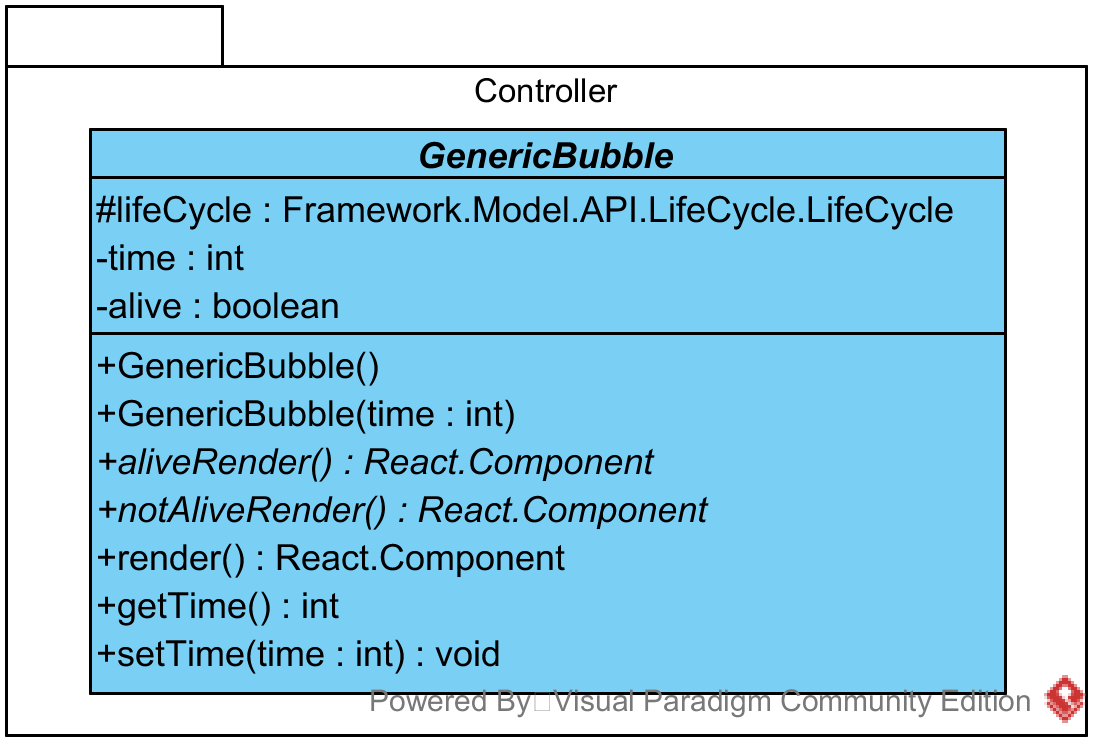
\includegraphics[width=10cm]{./diagrammi/framework/controller/genericbubble.png}
	\caption{Classe \class}
\end{figure}
\textbf{Descrizione:}\\
Classe astratta che collega la logica del Model alla resa grafica della View.

\textbf{Utilizzo:}\\
Viene utilizzata come base per creare le bubble.

\textbf{Classi ereditate:}
\begin{itemize}
	\item \code{React::Component}
\end{itemize}

\textbf{Sottoclassi:}
\begin{itemize}
	\item 
\end{itemize}

\textbf{Attributi:}
\begin{itemize}
	\item \field{\# lifeCycle: LifeCycle}: campo che permette di impostare il tempo di vita della bubble;
	\item \field{- time: int}: tempo di vita della bubble;
	\item \field{- alive: boolean}: indica se la bubble è in vita o meno.
\end{itemize}

\textbf{Metodi:}
\begin{itemize}
	\item \method{+ GenericBubble(props: Object[])}: costruttore della classe, inizializza gli attributi con le corrispondenti proprietà:
	\begin{itemize}
		\item \param{props: Object[]}: oggetto contenente tutte le proprietà passate al costruttore;
	\end{itemize}
	\item \method{\textit{+ aliveRender(): React::Component}}: renderizza la bubble mentre è in vita;
	\item \method{\textit{+ notAliveRender(): React::Component}}: renderizza la bubble a vita terminata;
	\item \method{+ render(): React::Component}: renderizza la bubble.
\end{itemize}

\setclass{Framework::View}
\subsubsection[::View]{\class}\label{\class}
\begin{figure}[H]
	\centering
	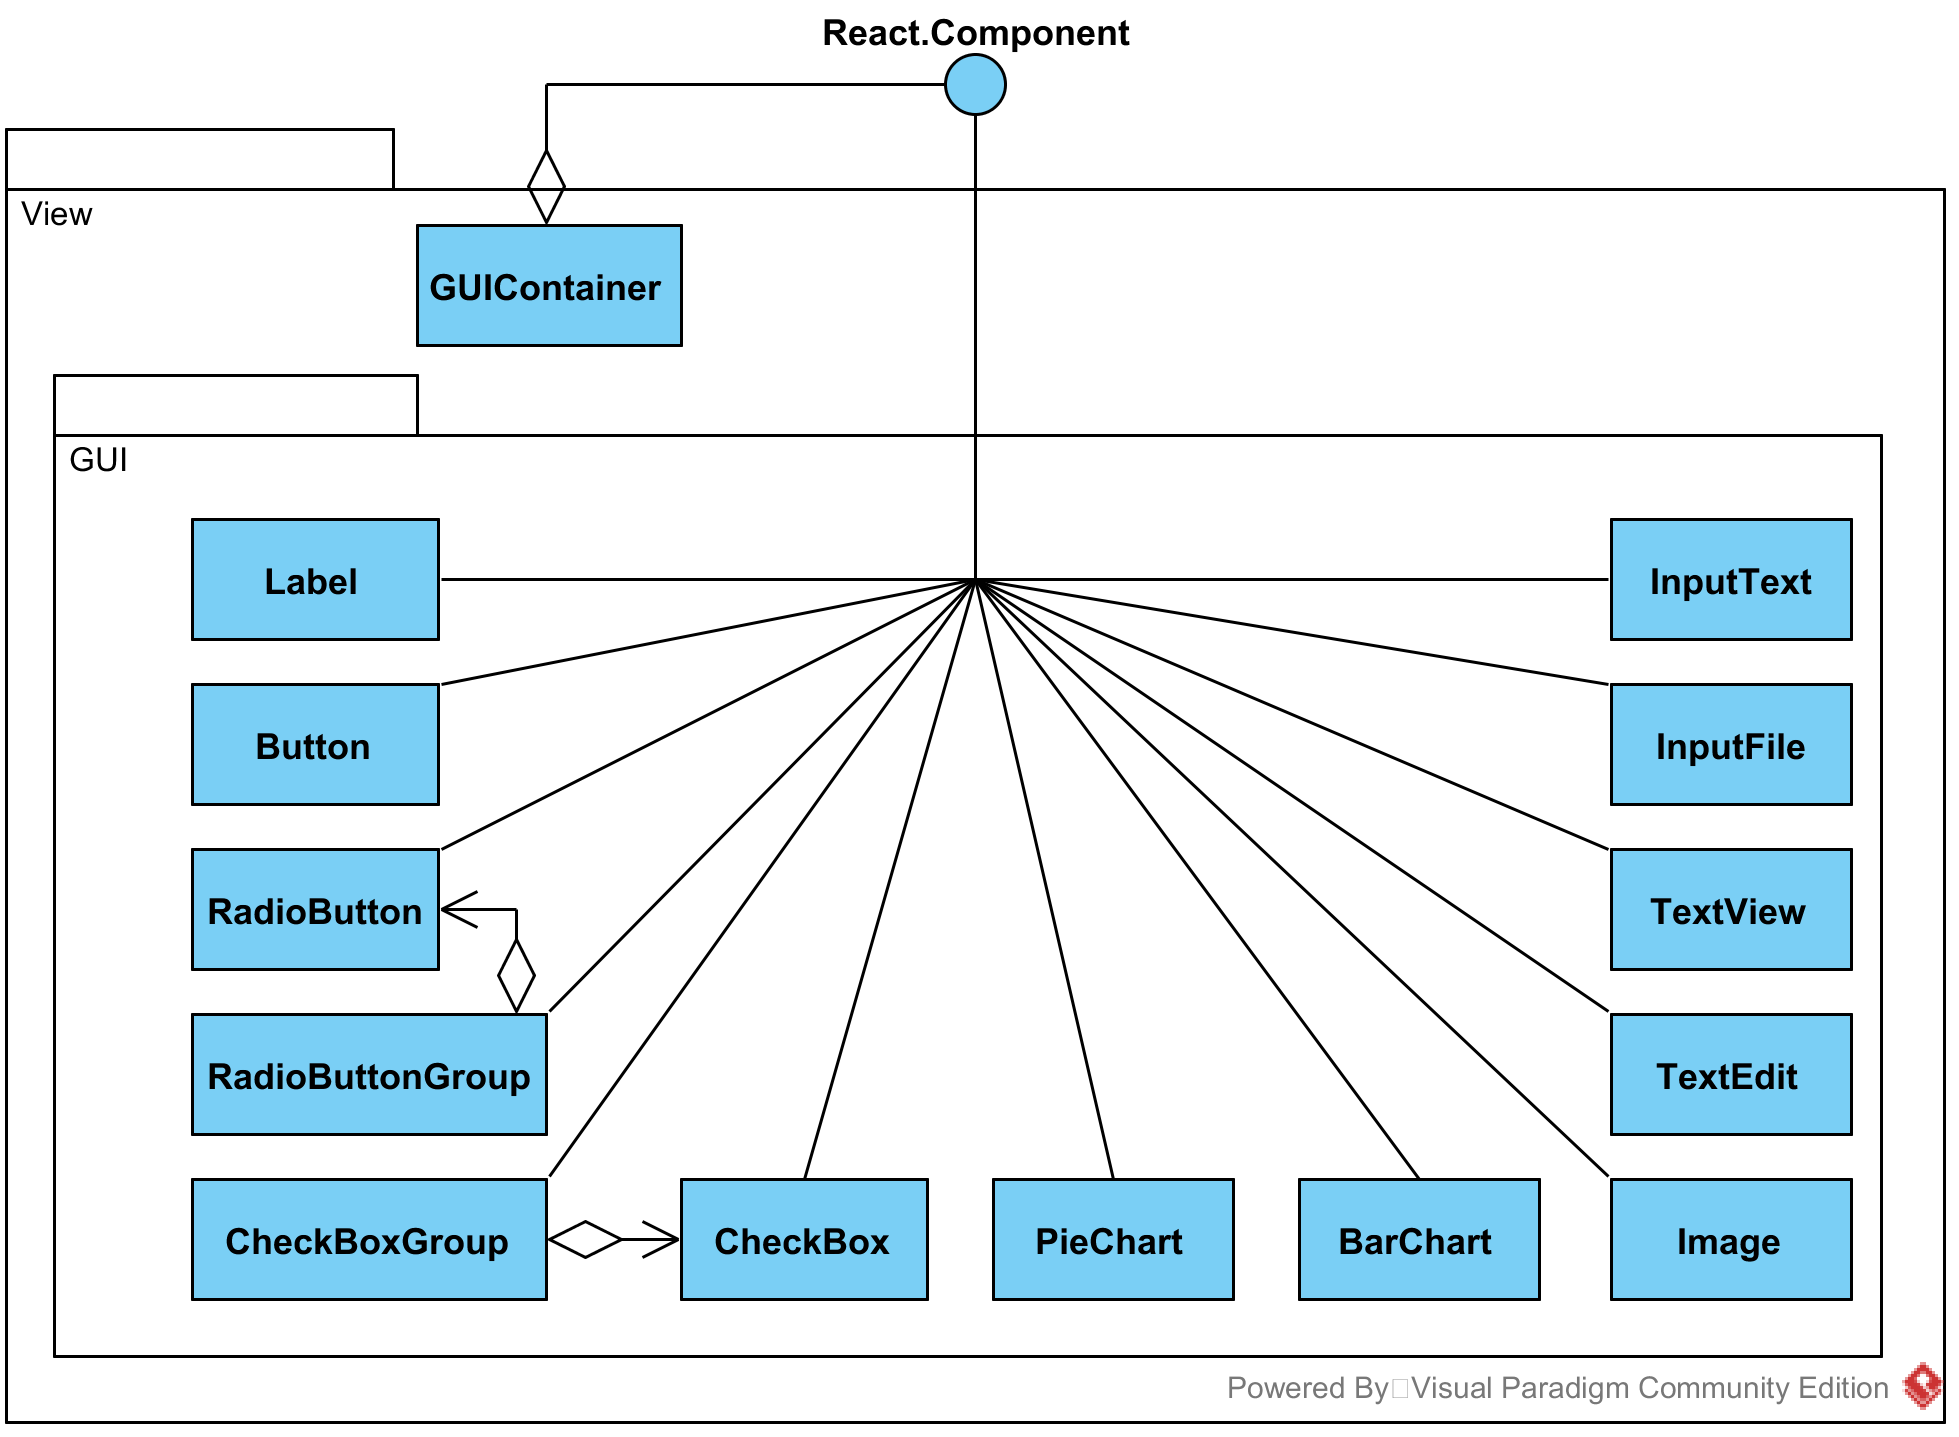
\includegraphics[width=15cm]{./diagrammi/framework/view.png}
	\caption{Classe \class}
\end{figure}
Il componente View è il contenitore principale per gli elementi grafici del framework. È composto al suo interno da un pattern Fa\c{c}ace sul sottosistema GUI e dalla classe GUIContainer che fa da contenitore per qualsiasi componente grafico.

\setclass{Framework::View::GUIContainer}
\paragraph[::GUIContainer]{\class}\mbox{}\\ \label{\class}
\begin{figure}[H]
	\centering
	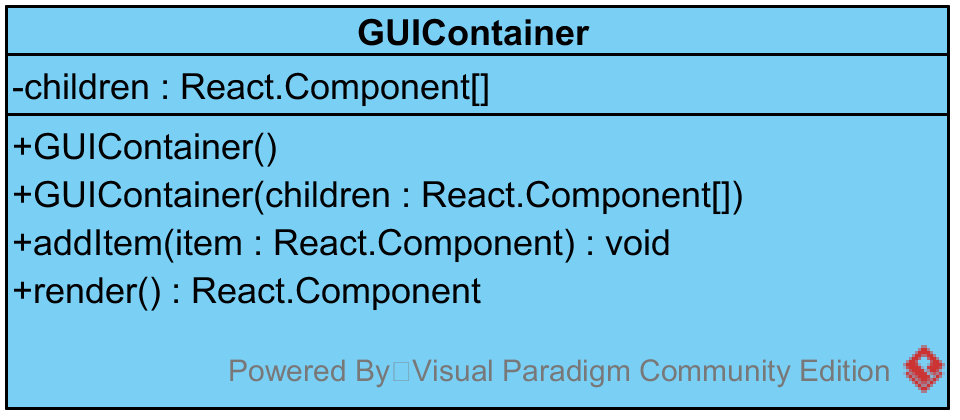
\includegraphics[width=7cm]{./diagrammi/framework/view/guicontainer.png}
	\caption{Classe \class}
\end{figure}
\textbf{Descrizione:}\\
Classe che rappresenta un generico contenitore per elementi grafici.

\textbf{Utilizzo:}\\
Viene utilizzato per raggruppare blocchi di elementi correlati tra loro.

\textbf{Classi ereditate:}
\begin{itemize}
	\item \code{React::Component}
\end{itemize}

%\textbf{Sottoclassi:}
%\begin{itemize}
%	\item 
%\end{itemize}

\textbf{Attributi:}
\begin{itemize}
	\item \field{- children: GUI[]}: array di componenti grafici.
\end{itemize}

\textbf{Metodi:}
\begin{itemize}
	\item \method{+ GUIContainer(props: Object[])}: costruttore della classe, inizializza gli attributi con le corrispondenti proprietà:
	\begin{itemize}
		\item \param{props: Object[]}: oggetto contenente tutte le proprietà passate al costruttore;
	\end{itemize}
	\item \method{+ render(): React::Component}: renderizza il contenitore.
\end{itemize}

\setclass{Framework::View::GUI::GUI}
\paragraph[::GUI]{\class}\mbox{}\\ \label{\class}
\begin{figure}[H]
	\centering
	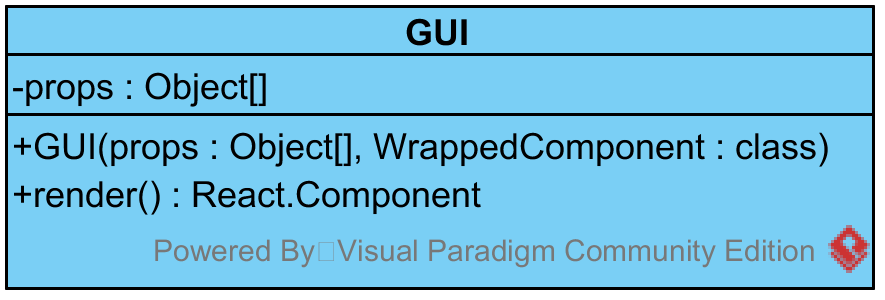
\includegraphics[width=9cm]{./diagrammi/framework/view/gui/gui.png}
	\caption{Classe \class}
\end{figure}
\textbf{Descrizione:}\\
Classe che rappresenta un generico elemento grafico. Implementa il design pattern Fa\c{c}ade.

\textbf{Utilizzo:}\\
Viene utilizzato per costruire gli elementi grafici.

\textbf{Classi ereditate:}
\begin{itemize}
	\item \code{React::Component}
\end{itemize}

%\textbf{Sottoclassi:}
%\begin{itemize}
%	\item 
%\end{itemize}

\textbf{Attributi:}
\begin{itemize}
	\item \field{- props: Object[]}: array contenente le proprietà del componente da creare.
\end{itemize}

\textbf{Metodi:}
\begin{itemize}
	\item \method{+ GUI(props: Object[], WrappedComponent: class)}: costruttore della classe, inizializza le proprietà del componente da creare:
	\begin{itemize}
		\item \param{props: Object[]}: oggetto contenente tutte le proprietà passate al costruttore;
		\item \param{WrappedComponent: class}: componente da creare;
	\end{itemize}
	\item \method{+ render(): React::Component}: renderizza il componente.
\end{itemize}

\setclass{Framework::View::GUI::BarChart}
\paragraph[::BarChart]{\class}\mbox{}\\ \label{\class}
\begin{figure}[H]
	\centering
	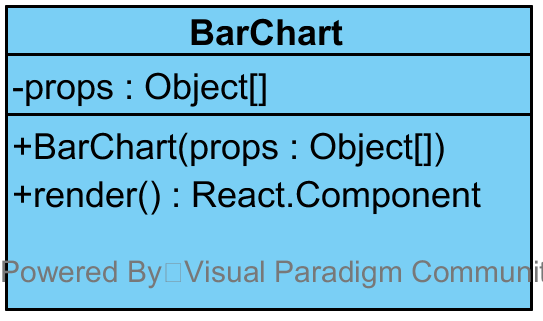
\includegraphics[width=7cm]{./diagrammi/framework/view/gui/barchart.png}
	\caption{Classe \class}
\end{figure}
\textbf{Descrizione:}\\
Classe che rappresenta un grafico a istogramma.

%\textbf{Utilizzo:}\\
%Viene utilizzato per costruire gli elementi grafici.

\textbf{Classi ereditate:}
\begin{itemize}
	\item \code{Rechart::BarChart}
\end{itemize}

%\textbf{Sottoclassi:}
%\begin{itemize}
%	\item 
%\end{itemize}

\textbf{Attributi:}
\begin{itemize}
	\item \field{- props: Object[]}: proprietà della classe.
\end{itemize}

\textbf{Metodi:}
\begin{itemize}
	\item \method{+ BarChart(props: Object[])}: costruttore, assegna le proprietà;
	\begin{itemize}
		\item \param{props: Object[]}: array di oggetti contenenti le proprietà;
	\end{itemize}
	\item \method{+ render(): React::Component}: renderizza il componente.
\end{itemize}

\setclass{Framework::View::GUI::Button}
\paragraph[::Button]{\class}\mbox{}\\ \label{\class}
\begin{figure}[H]
	\centering
	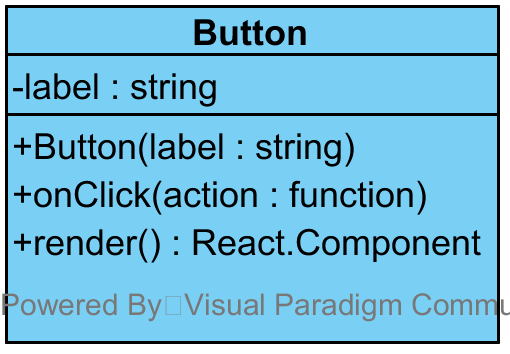
\includegraphics[width=7cm]{./diagrammi/framework/view/gui/button.png}
	\caption{Classe \class}
\end{figure}
\textbf{Descrizione:}\\
Classe che rappresenta un bottone.

\textbf{Utilizzo:}\\
Viene utilizzato per i bottoni generici all'interno della bubble.

\textbf{Classi ereditate:}
\begin{itemize}
	\item \code{React::Component}
\end{itemize}

%\textbf{Sottoclassi:}
%\begin{itemize}
%	\item 
%\end{itemize}

\textbf{Attributi:}
\begin{itemize}
	\item \field{- props: Object[]}: array contenente le proprietà.
\end{itemize}

\textbf{Metodi:}
\begin{itemize}
	\item \method{+ Button(props: Object[])}: costruttore della classe, assegna le proprietà:
	\begin{itemize}
		\item \param{props: Object[]}: array di oggetti contenenti le proprietà;
	\end{itemize}
	\item \method{+ render(): React::Component}: renderizza il componente.
\end{itemize}

\setclass{Framework::View::GUI::CheckBox}
\paragraph[::CheckBox]{\class}\mbox{}\\ \label{\class}
\begin{figure}[H]
	\centering
	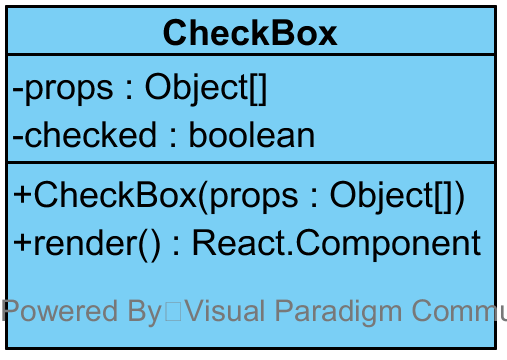
\includegraphics[width=7cm]{./diagrammi/framework/view/gui/checkbox.png}
	\caption{Classe \class}
\end{figure}
\textbf{Descrizione:}\\
Classe che rappresenta una checkbox.

\textbf{Utilizzo:}\\
Viene utilizzata per costruire gli elementi della to-do list.

\textbf{Classi ereditate:}
\begin{itemize}
	\item \code{React::Component}
\end{itemize}

%\textbf{Sottoclassi:}
%\begin{itemize}
%	\item 
%\end{itemize}

\textbf{Attributi:}
\begin{itemize}
	\item \field{- props: Object[]}: array contenente le proprietà della classe;
	\item \field{- checked: boolean}: indica lo stato della checkbox.
\end{itemize}

\textbf{Metodi:}
\begin{itemize}
	\item \method{+ CheckBox(props: Object[])}: costruttore della classe, assegna le proprietà:
	\begin{itemize}
		\item \param{props: Object[]}: array contenente le proprietà della classe;
	\end{itemize}
	\item \method{+ render(): React::Component}: renderizza il componente.
\end{itemize}

\setclass{Framework::View::CheckBoxGroup}
\paragraph[::CheckBoxGroup]{\class}\mbox{}\\ \label{\class}
\begin{figure}[H]
	\centering
	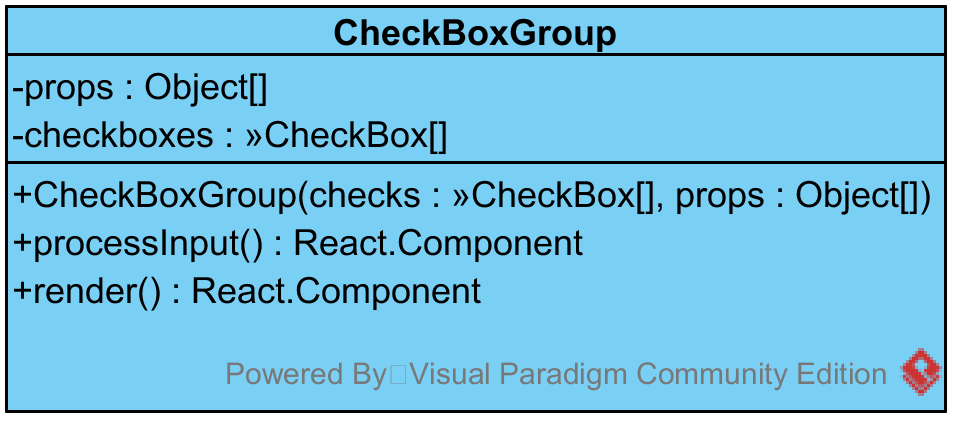
\includegraphics[width=10cm]{./diagrammi/framework/view/gui/checkboxgroup.png}
	\caption{Classe \class}
\end{figure}
\textbf{Descrizione:}\\
Classe che rappresenta una contenitore di checkbox.

\textbf{Utilizzo:}\\
Viene utilizzata per racchiudere gli elementi della to-do list.

\textbf{Classi ereditate:}
\begin{itemize}
	\item \code{React::Component}
\end{itemize}

%\textbf{Sottoclassi:}
%\begin{itemize}
%	\item 
%\end{itemize}

\textbf{Attributi:}
\begin{itemize}
	\item \field{- checks: CheckBox[]}: array contenente le checkbox;
	\item \field{- props: Object[]}: array contenente le proprietà della classe.
\end{itemize}

\textbf{Metodi:}
\begin{itemize}
	\item \method{+ CheckBoxGroup(checks: CheckBox[], props: Object[])}: costruttore della classe, assegna le proprietà:
	\begin{itemize}
		\item \param{checks: CheckBox[]}: array contenente le checkbox;
		\item \param{props: Object[]}: array contenente le proprietà della classe;
	\end{itemize}
	\item \method{+ processInput(): React::Component}: renderizza i singoli componenti CheckBox;
	\item \method{+ render(): React::Component}: renderizza il componente.
\end{itemize}

\setclass{Framework::View::Image}
\paragraph[::Image]{\class}\mbox{}\\ \label{\class}
\begin{figure}[H]
	\centering
	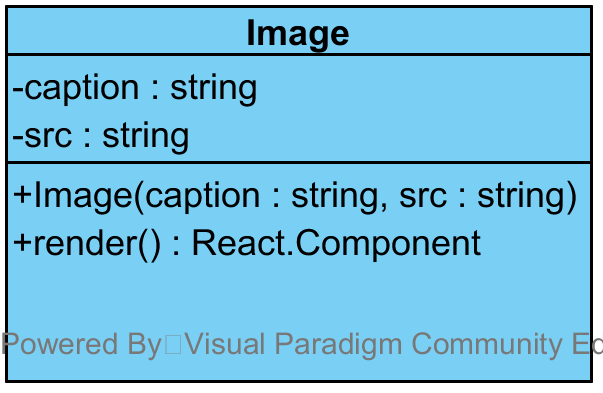
\includegraphics[width=7cm]{./diagrammi/framework/view/gui/image.png}
	\caption{Classe \class}
\end{figure}
\textbf{Descrizione:}\\
Classe che rappresenta una immagine.

\textbf{Utilizzo:}\\
Viene utilizzata per inserire qualsiasi tipo di immagine.

\textbf{Classi ereditate:}
\begin{itemize}
	\item \code{React::Component}
\end{itemize}

%\textbf{Sottoclassi:}
%\begin{itemize}
%	\item 
%\end{itemize}

\textbf{Attributi:}
\begin{itemize}
	\item \field{- caption: string}: descrizione testuale dell'immagine;
	\item \field{- src: string}: URI dell'immagine.
\end{itemize}

\textbf{Metodi:}
\begin{itemize}
	\item \method{+ Image(caption: string, src: string)}: costruttore della classe, assegna gli attributi:
	\begin{itemize}
		\item \param{caption: string}: descrizione testuale dell'immagine;
		\item \param{src: string}: URI dell'immagine;
	\end{itemize}
	\item \method{+ render(): React::Component}: renderizza il componente.
\end{itemize}

\setclass{Framework::View::InputFile}
\paragraph[::InputFile]{\class}\mbox{}\\ \label{\class}
\begin{figure}[H]
	\centering
	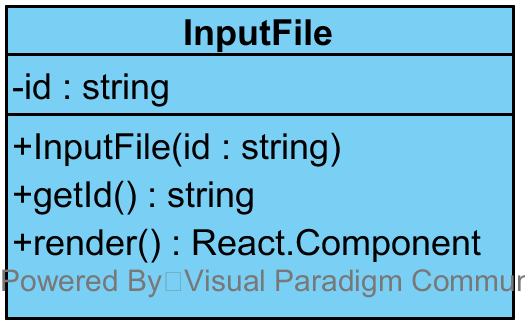
\includegraphics[width=7cm]{./diagrammi/framework/view/gui/inputfile.png}
	\caption{Classe \class}
\end{figure}
\textbf{Descrizione:}\\
Classe che permette di caricare un file.

\textbf{Utilizzo:}\\
Viene utilizzata per caricare file.

\textbf{Classi ereditate:}
\begin{itemize}
	\item \code{React::Component}
\end{itemize}

%\textbf{Sottoclassi:}
%\begin{itemize}
%	\item 
%\end{itemize}

\textbf{Attributi:}
\begin{itemize}
	\item \field{- id: string}: id dell'input;
\end{itemize}

\textbf{Metodi:}
\begin{itemize}
	\item \method{+ InputFile(id: string)}: costruttore della classe, assegna l'id:
	\begin{itemize}
		\item \param{id: string}: id da assegnare;
	\end{itemize}
	\item \method{+ render(): React::Component}: renderizza il componente.
\end{itemize}

\setclass{Framework::View::InputText}
\paragraph[::InputText]{\class}\mbox{}\\ \label{\class}
\begin{figure}[H]
	\centering
	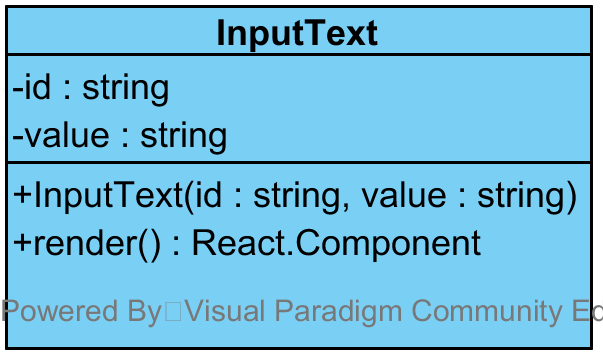
\includegraphics[width=7cm]{./diagrammi/framework/view/gui/inputtext.png}
	\caption{Classe \class}
\end{figure}
\textbf{Descrizione:}\\
Classe che rappresenta un form di inserimento testo.

\textbf{Utilizzo:}\\
Viene utilizzata per permettere raccogliere informazioni testuali inserite dall'utente.

\textbf{Classi ereditate:}
\begin{itemize}
	\item \code{React::Component}
\end{itemize}

%\textbf{Sottoclassi:}
%\begin{itemize}
%	\item 
%\end{itemize}

\textbf{Attributi:}
\begin{itemize}
	\item \field{- id: string}: id dell'input;
	\item \field{- value: string}: testo di default.
\end{itemize}

\textbf{Metodi:}
\begin{itemize}
	\item \method{+ InputText(id: string, value: string)}: costruttore della classe, assegna gli attributi:
	\begin{itemize}
		\item \param{id: string}: id da assegnare al componente;
		\item \param{value: string}: valore da visualizzare;
	\end{itemize}
	\item \method{+ render(): React::Component}: renderizza il componente.
\end{itemize}

\setclass{Framework::View::Label}
\paragraph[::Label]{\class}\mbox{}\\ \label{\class}
\begin{figure}[H]
	\centering
	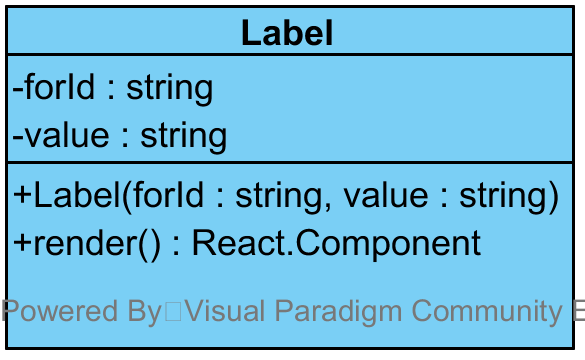
\includegraphics[width=7cm]{./diagrammi/framework/view/gui/label.png}
	\caption{Classe \class}
\end{figure}
\textbf{Descrizione:}\\
Classe che rappresenta una label per un generico campo di inserimento dati.

\textbf{Utilizzo:}\\
Viene utilizzata assieme ai campi input per assegnarci un'etichetta descrittiva.

\textbf{Classi ereditate:}
\begin{itemize}
	\item \code{React::Component}
\end{itemize}

%\textbf{Sottoclassi:}
%\begin{itemize}
%	\item 
%\end{itemize}

\textbf{Attributi:}
\begin{itemize}
	\item \field{- forId: string}: id del componente input associato;
	\item \field{- value: string}: descrizione del componente input.
\end{itemize}

\textbf{Metodi:}
\begin{itemize}
	\item \method{+ Label(forId: string, value: string)}: costruttore della classe, assegna gli attributi:
	\begin{itemize}
		\item \param{forId: string}: id del componente input da descrivere;
		\item \param{value: string}: descrizione dell'input da immettere;
	\end{itemize}
	\item \method{+ render(): React::Component}: renderizza il componente.
\end{itemize}

\setclass{Framework::View::PieChart}
\paragraph[::PieChart]{\class}\mbox{}\\ \label{\class}
\begin{figure}[H]
	\centering
	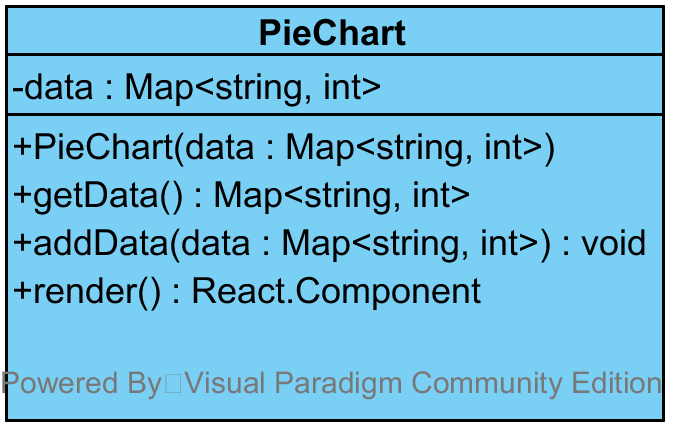
\includegraphics[width=7cm]{./diagrammi/framework/view/gui/piechart.png}
	\caption{Classe \class}
\end{figure}
\textbf{Descrizione:}\\
Classe che rappresenta un grafico a torta.

%\textbf{Utilizzo:}\\
%Viene utilizzata per inserire qualsiasi tipo di immagine.

\textbf{Classi ereditate:}
\begin{itemize}
	\item \code{Rechart::PieChart}
\end{itemize}

%\textbf{Sottoclassi:}
%\begin{itemize}
%	\item 
%\end{itemize}

\textbf{Attributi:}
\begin{itemize}
	\item \field{- props: Object[]}: proprietà della classe.
\end{itemize}

\textbf{Metodi:}
\begin{itemize}
	\item \method{+ PieChart(props: Object[])}: costruttore della classe, assegna le proprietà:
	\begin{itemize}
		\item \param{props: Object[]}: proprietà dell'oggetto da costruire;
	\end{itemize}
	\item \method{+ render(): React::Component}: renderizza il componente.
\end{itemize}

\setclass{Framework::View::RadioButton}
\paragraph[::RadioButton]{\class}\mbox{}\\ \label{\class}
\begin{figure}[H]
	\centering
	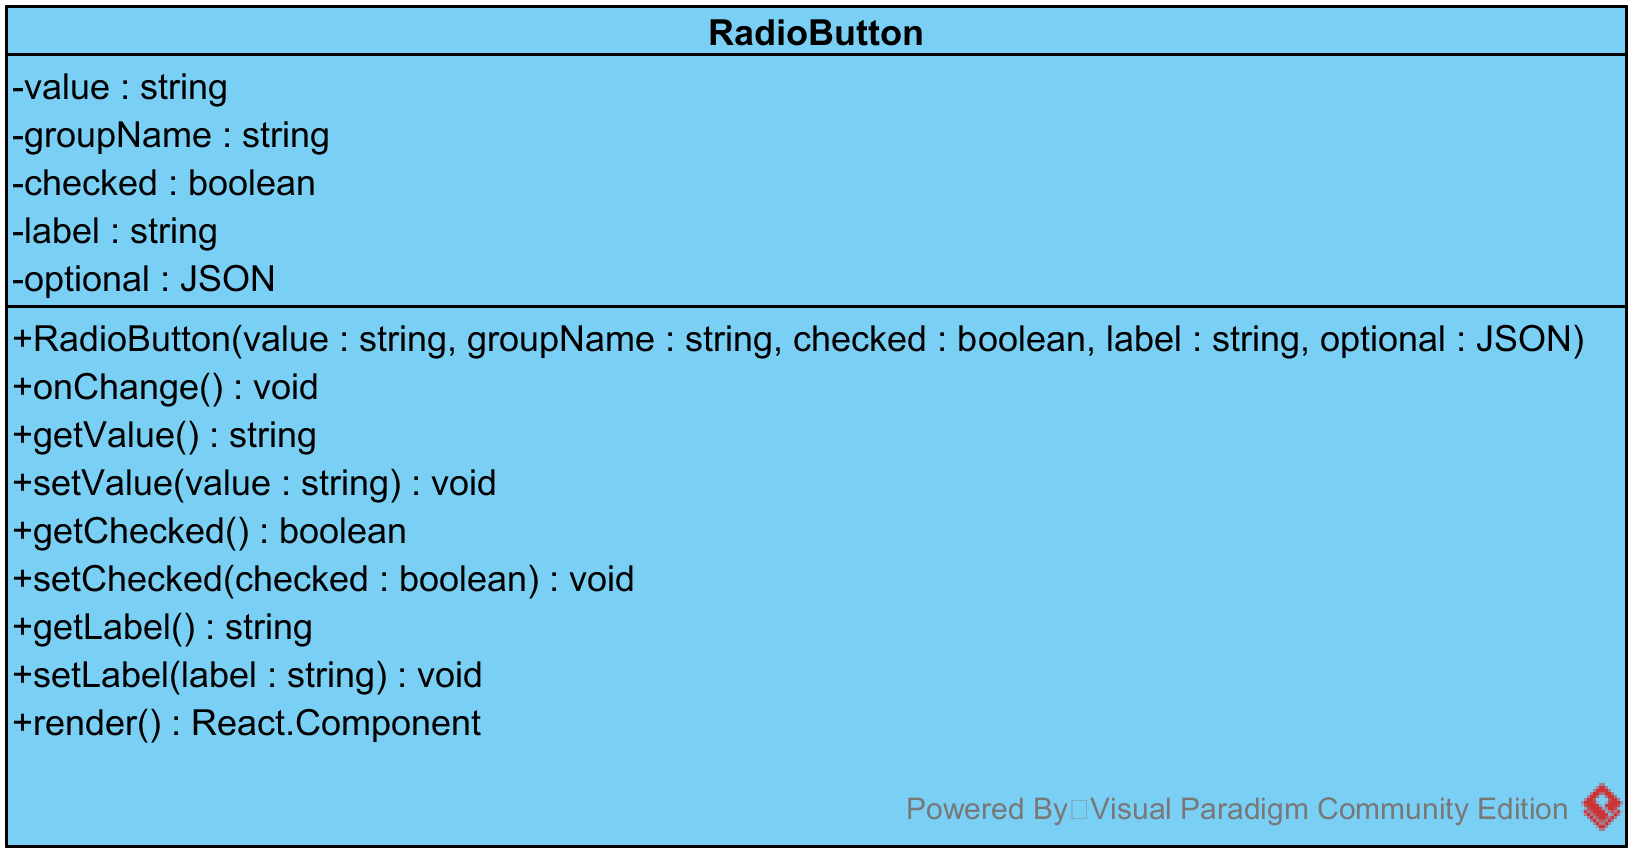
\includegraphics[width=14cm]{./diagrammi/framework/view/gui/radiobutton.png}
	\caption{Classe \class}
\end{figure}
\textbf{Descrizione:}\\
Classe che rappresenta una bottone radio.

\textbf{Utilizzo:}\\
Viene utilizzata per i bottoni radio all'interno della bubble.

\textbf{Classi ereditate:}
\begin{itemize}
	\item \code{React::Component}
\end{itemize}

%\textbf{Sottoclassi:}
%\begin{itemize}
%	\item 
%\end{itemize}

\textbf{Attributi:}
\begin{itemize}
	\item \field{- value: string}: valore del bottone;
	\item \field{- groupName: string}: identificativo del gruppo di bottoni di appartenenza;
	\item \field{- checked: boolean}: stato di selezione;
	\item \field{- label: string}: descrizione testuale del bottone;
	\item \field{- optional: Object[]}: array contenente proprietà opzionali.
\end{itemize}

\textbf{Metodi:}
\begin{itemize}
	\item \method{+ RadioButton(value: string, groupName: string, checked: boolean, label: string, optional: Object[])}: costruttore della classe, assegna gli attributi:
	\begin{itemize}
		\item \param{value: string}: valore del bottone;
		\item \param{groupName: string}: nome del gruppo di appartenenza;
		\item \param{checked: boolean}: setta il bottone come selezionato se true (solo uno per gruppo dovrebbe avere questo parametro a true);
		\item \param{label: string}: descrizione testuale del bottone;
		\item \param{optional: Object[]}: array di oggetti contenente proprietà opzionali;
	\end{itemize}
	\item \method{+ onChange(): void}: comportamento da adottare quando lo stato \texttt{checked} varia;
	\item \method{+ render(): React::Component}: renderizza il componente.
\end{itemize}

\setclass{Framework::View::RadioButtonGroup}
\paragraph[::RadioButtonGroup]{\class}\mbox{}\\ \label{\class}
\begin{figure}[H]
	\centering
	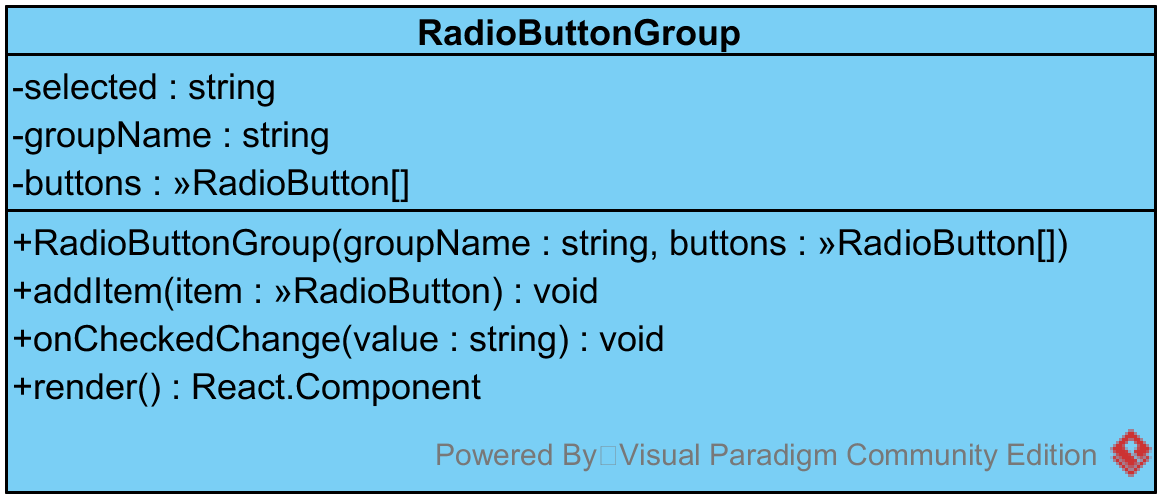
\includegraphics[width=10cm]{./diagrammi/framework/view/gui/radiobuttongroup.png}
	\caption{Classe \class}
\end{figure}
\textbf{Descrizione:}\\
Classe che rappresenta un contenitore per bottoni radio.

\textbf{Utilizzo:}\\
Viene utilizzata nella bubble per raggruppare bottoni radio affini.

\textbf{Classi ereditate:}
\begin{itemize}
	\item \code{React::Component}
\end{itemize}

%\textbf{Sottoclassi:}
%\begin{itemize}
%	\item 
%\end{itemize}

\textbf{Attributi:}
\begin{itemize}
	\item \field{- selected: string}: valore del bottone selezionato;
	\item \field{- groupName: string}: nome identificativo del gruppo;
	\item \field{- buttons: RadioButton[]}: array di bottoni radio appartenenti al gruppo;
\end{itemize}

\textbf{Metodi:}
\begin{itemize}
	\item \method{+ RadioButtonGroup(groupName: string, buttons: RadioButton[])}: costruttore della classe, assegna gli attributi:
	\begin{itemize}
		\item \param{groupName: string}: nome del gruppo;
		\item \param{buttons: RadioButton[]}: insieme di bottoni radio da assegnare all'istanza del gruppo;
	\end{itemize}
	\item \method{+ onCheckedChange(value: string): void}: aggiorna il valore di \texttt{selected};
	\item \method{+ render(): React::Component}: renderizza il componente.
\end{itemize}


\setclass{Framework::View::TextEdit}
\paragraph[::TextEdit]{\class}\mbox{}\\ \label{\class}
\begin{figure}[H]
	\centering
	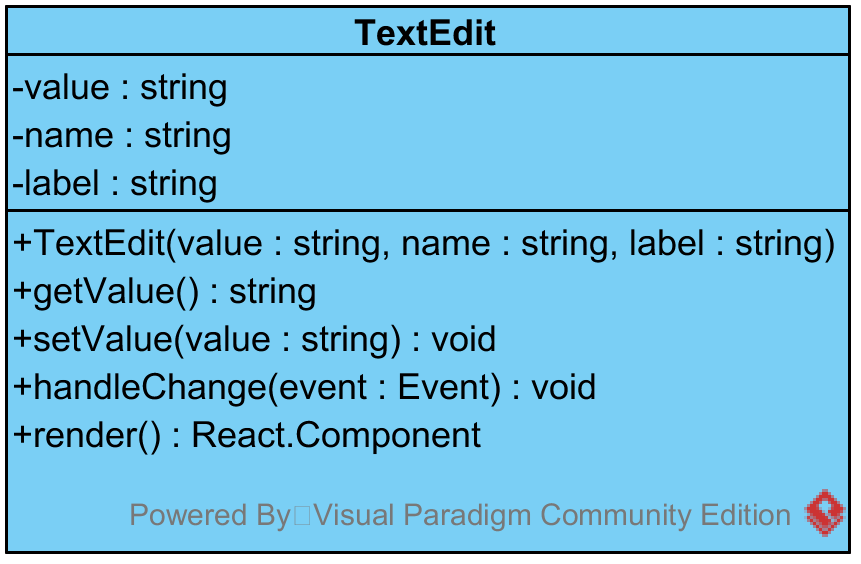
\includegraphics[width=9cm]{./diagrammi/framework/view/gui/textedit.png}
	\caption{Classe \class}
\end{figure}
\textbf{Descrizione:}\\
Classe che rappresenta un campo di testo modificabile.

\textbf{Utilizzo:}\\
Viene utilizzata per permettere l'inserimento di più righe di testo.

\textbf{Classi ereditate:}
\begin{itemize}
	\item \code{React::Component}
\end{itemize}

%\textbf{Sottoclassi:}
%\begin{itemize}
%	\item 
%\end{itemize}

\textbf{Attributi:}
\begin{itemize}
	\item \field{- value: string}: valore di default del testo;
	\item \field{- name: string}: identificativo del campo di testo;
	\item \field{- label: string}: descrizione testuale dell'input.
\end{itemize}

\textbf{Metodi:}
\begin{itemize}
	\item \method{+ TextEdit(value: string, name: string, label: string)}: costruttore della classe, assegna gli attributi:
	\begin{itemize}
		\item \param{value: string}: descrizione testuale dell'input;
		\item \param{name: string}: identificativo del campo di testo;
		\item \param{label: string}: descrizione testuale dell'input;
	\end{itemize}
	\item \method{+ handleChange(event: Event): void}: aggiorna lo stato del componente;
	\item \method{+ render(): React::Component}: renderizza il componente.
\end{itemize}


\setclass{Framework::View::TextView}
\paragraph[::TextView]{\class}\mbox{}\\ \label{\class}
\begin{figure}[H]
	\centering
	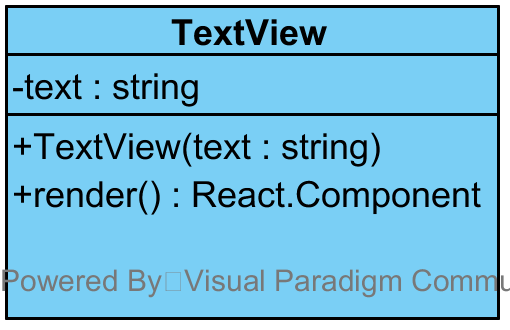
\includegraphics[width=7cm]{./diagrammi/framework/view/gui/textview.png}
	\caption{Classe \class}
\end{figure}
\textbf{Descrizione:}\\
Classe che visualizza del testo non modificabile.

\textbf{Utilizzo:}\\
Viene utilizzata per mostrare testo generico.

\textbf{Classi ereditate:}
\begin{itemize}
	\item \code{React::Component}
\end{itemize}

%\textbf{Sottoclassi:}
%\begin{itemize}
%	\item 
%\end{itemize}

\textbf{Attributi:}
\begin{itemize}
	\item \field{- text: string}: testo visualizzato.
\end{itemize}

\textbf{Metodi:}
\begin{itemize}
	\item \method{+ TextView(text: string)}: costruttore della classe:
	\begin{itemize}
		\item \param{text: string}: testo da visualizzare.
	\end{itemize}
	\item \method{+ render(): React::Component}: renderizza il componente.
\end{itemize}
